\documentclass[18pt, a1paper, portrait]{tikzposter}
\usetikzlibrary{fit,arrows,tikzmark,shadows,calc,automata}
\newcommand\NameBlock[1]{\node[fit=(blockbody)(blocktitle),inner sep=5pt] (#1) {};}
\usepackage[utf8]{inputenc}
\usepackage{subcaption}
\usepackage{adjustbox}
\usepackage{booktabs}

\usepackage[backend=bibtex]{biblatex}
\addbibresource{poster.bib}

\usepackage{authblk}
\makeatletter
% revert \maketitle to its old definition
% \def\maketitle{\AB@maketitle}
\renewcommand\maketitle{\AB@maketitle}

% put affiliations into one line
\renewcommand\AB@affilsepx{\quad\protect\Affilfont}
%
\makeatother
% set font for affiliations
\renewcommand\Affilfont{\Large}


\tikzposterlatexaffectionproofoff

% \usepackage{poster-style}
\usepackage{filecontents}
\usepackage{listings}

\bibliography{references}


\title{FAT-Pointer based range TLB}
% \author{}
\date{\today}
% \institute{Heriot-Watt University UK \and Université de Toulouse France,
% and Carleton University Canada}

\author[1]{\Large Akilan Selvacoumar}
\author[1]{ Robert Stewart}
\author[1]{ Hans-Wolfgang Loidl}
\author[1]{ Ryad Soobhany}
\affil[1]{Heriot-Watt University, UK}

% \titlegraphic{
% 
\includegraphics[width=0.1\paperwidth]{hw-logo.png}
% }

\usepackage{blindtext}
\usepackage{comment}

% Default, Rays, Basic, Simple, Envelope, Wave, Board, Autumn, Desert
%
% good: Default, Basic, Simple
\usetheme{Basic}

% \renewcommand{\titleposright}{50mm}
% \titleposright=100mm
\definetitlestyle{sampletitle}{
  innersep=-10pt,
  titletotopverticalspace=-400mm,
  titletoblockverticalspace=10mm
}
{}

\usetitlestyle{sampletitle}
% \titleposleft=-300mm

% \usetitlestyle[titletotopverticalspace=-50mm,]{Basic}


% Britain, Australia, Sweden, Spain,Russia,Denmark,Germany
\usecolorstyle{Default}



\begin{document}
%   SICSA Postdoctoral and Early Career Researcher Exchanges.};

% removes space at top
\maketitle[titletotopverticalspace=-5mm]
% \maketitle

% \block{~}
% {
% \blindtext
% }

\begin{columns}
  \column{0.5}

  \block{Abstract}{

    % \begin{minipage}[t]{0.6\linewidth}

      \begin{tikzfigure}
        % \includegraphics[width=0.4\textwidth]{images/abstraction-poster.jpg}
      \end{tikzfigure}
      Capability-based addressing in the CHERI architecture is designed to improve hardware-level system security. These security guarantees 
      can degrade runtime performance due to increased L1 TLB misses \cite{1}. Our aim is to achieve capability-based security 
      at zero performance cost. We will use fat pointers to simplify and implement a recently proposed range TLB scheme \cite{2}, 
      with the goal of reducing L1 TLB misses and page-walks for memory-intensive CHERI workloads.
% The FAT pointer structure of CHERI allows to encode custom bits of meta-data which in this
% case can be used to store the ID of the range TLB entry.

% (This would inturn lookup TLB entries in the range table rather than looking up the L1 TLB entry)



    \vspace{0.5cm}
  }

  \block{Research Questions}{

    % \hspace{0.5cm}

    \begin{minipage}[t]{1\linewidth}
      \textbf{\textit{Research Questions:}}
      \begin{itemize}
        \item (RQ1) Can L1 misses and page-walks be reduced for memory intensive CHERI workloads?
        \item (RQ2) Is it possible to implement a simple Range TLB scheme with 8 bits using region of a fat pointer?
        \item (RQ3) Can fat pointer based address translation lower the runtime overheads of hardware-level security in capability hardware like CHERI?
        % monolithic OS or containers in terms of wall-clock runtimes, CPU
        % profiling and memory profiling?
      % \item \textit{parallelising actors can increase throughput}
      \end{itemize}

    \end{minipage}%
    % \hspace{0.2cm}

    % \vspace{0.1cm}

    % \begin{tikzfigure}
    %   % \includegraphics[width=0.4\textwidth]{images/parallel-layers-poster.png}
    % \end{tikzfigure}

    % \vspace{-0.5cm}
  }

\column{0.5}

  \NameBlock{transformation}
  \block{Our Approach}{
    % \vspace{0.7cm}
    % \hspace{0.4cm}

    % \begin{minipage}[t]{0.4\linewidth}
    %   \vspace{-0.9cm}
    %   \begin{tikzfigure}{}
    %     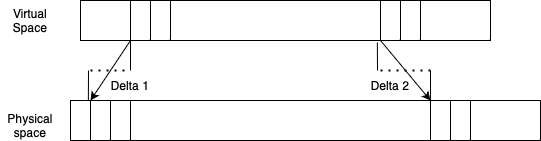
\includegraphics[width=2.47\textwidth]{RangeTranlations.drawio.png}
    %   \end{tikzfigure}
    % \end{minipage}

    Range translation is the process of mapping between contigous virtual pages mapped 
    to contigous phyiscal pages \cite{3}. Recent work on FlexPointer\cite{2} extended RMM\cite{3}
    by encoding RangeIDs to the remaining 16 bits on a 64-bit virtual address.
    In the absence of fat pointers, their Range TLB was its own data structure in memory.
    We use fat pointers to simplify the implementation of Range TLB by using the bounds metadata
    to extract the lower and upper bounds which inturns allows us to encode the offset to the 
    Pointer to map to the Physical page number. We hope to reproduce the FlexPointer results of 
    reducing L1 tlb misses and page walks.


    % The current expirement adopts the range translation concept from
    % FlexPointer[1] which was inturn adopted from RMM[2]. A range consists 
    % of contigous virtual and phyiscal pages. Addresses share a 
    % common Delta. To assume 
    % physical contiguity of a particular range we are proposing 
    % to use eager paging strategy as proposed from FlexPointer[1].

%     How about a "Our Idea" box, with an argumentation sequence (written by you as a paragraph) could be:

% Range translation is the process of , e.g. RMM [cite].

% Recent work on FlexPointer [cite] extended RMM .

% In the absence of fat pointers, their Range TLB was its own data structure in memory.

% We use fat pointers to simplify the implementation of Range TLB by using .

% We believe this simplified will <state very clearly and succinctly why you think step 4 will result in better performance than FlexPointer.

% alternatively, if you think it's not about beating FlexPointer but instead making CHERI faster in purecap mode, then...

% We hope to reproduce the FlexPointer results of reducing L1 misses and page walks, to remove recently observed for performance degredation -- the cost of hardware-level security.

    % The current expirement adopts the range translation concept from
    % FlexPointer[1] which was inturn adopted from RMM[2]. A range consists 
    % of contigous virtual and phyiscal pages. Addresses share a 
    % common Delta. To assume 
    % physical contiguity of a particular range we are proposing 
    % to use eager paging strategy as proposed from FlexPointer[1].

    % \begin{minipage}[t]{0.4\linewidth}
    %   \vspace{-0.9cm}
    %   \begin{tikzfigure}{}
    %     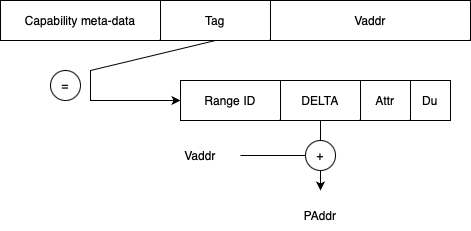
\includegraphics[width=2.47\textwidth]{RangeTLB.drawio.png}
    %   \end{tikzfigure}
    % \end{minipage}
    % \vspace{0.5cm}
    % \vspace{0.7cm}

    % Range TLB is organised as a fully associative cache, As per the
    % conventional the page table the lower 12 bits is used record
    % attributes (eg: R/W: Read/Write). 

    % \begin{minipage}[t]{0.4\linewidth}
    %   \vspace{-0.9cm}
    %   \begin{tikzfigure}{}
    %     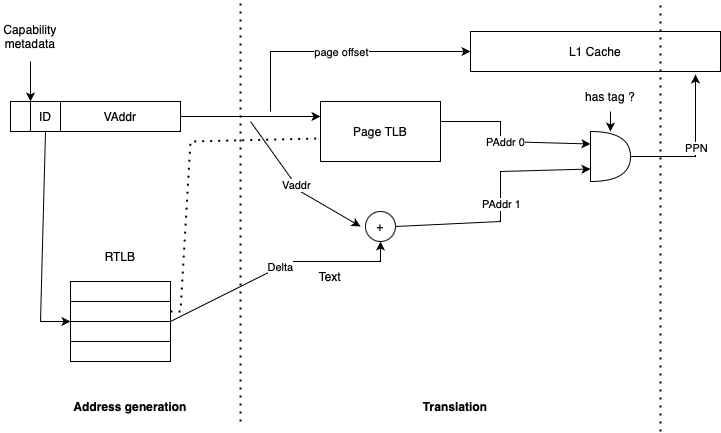
\includegraphics[width=2.47\textwidth]{Hardwareoverview.drawio.png}
    %   \end{tikzfigure}
    % \end{minipage}
    \vspace{0.5cm}
    \vspace{0.7cm}
    
    % Since the Range ID does not participate in the address generation. Using 
    % the ID provided the search for the delta value can occur on parallel to 
    % the address generation. Due to this the range TLB is shifted to a 
    % earlier stage.
 }

  \NameBlock{transformation}
  \block{References}{
    % \hspace{0.4cm}
      % monolithic OS or containers in terms of wall-clock runtimes, CPU
      % profiling and memory profiling?
    % \column{1}

    \begin{thebibliography}{9}
      \bibitem{1}Bramley, J., Jacob, D., Lascu, A., Singer, J. \& Tratt, L. Picking a CHERI Allocator: Security and Performance Considerations. {\em Proceedings Of The 2023 ACM SIGPLAN International Symposium On Memory Management}. (2023,6), https://doi.org/10.1145%252F3591195.3595278
      \bibitem{2}Chen, D., Tong, D., Yang, C., Yi, J. \& Cheng, X. FlexPointer: Fast Address Translation Based on Range TLB and Tagged Pointers. {\em ACM Trans. Archit. Code Optim.}. \textbf{20} (2023,3), https://doi.org/10.1145/3579854
      \bibitem{3}Karakostas, V., Gandhi, J., Ayar, F., Cristal, A., Hill, M., McKinley, K., Nemirovsky, M., Swift, M. \& Ünsal, O. Redundant Memory Mappings for Fast Access to Large Memories. {\em SIGARCH Comput. Archit. News}. \textbf{43}, 66-78 (2015,6), https://doi.org/10.1145/2872887.2749471
      \end{thebibliography}

      \column{1}
      \begin{minipage}[t]{0.4\linewidth}
        \vspace{-0.9cm}
        \begin{tikzfigure}{}
          
\includegraphics[width=0.6\textwidth]{Repo-url.png}
        \end{tikzfigure}
      \end{minipage}
      \column{0.5}



 }

  %   \NameBlock{transformation}
  %   \block{References}{
  %     \hspace{0.4cm}

  %   %  \begin{itemize}
  %   %    \item Building a parallel benchmark suite for Unikernels.
  %   %    \item Analysing the metrics provided by the Go compiler such as Heap usage, Number OS threads created by run time etc…
  %   %    \item Benchmarking other Unikernel implementation using the benchmark suite (1)
  %   %  \end{itemize}



  %  }


  % \NameBlock{results}
  % \block{Experimental Setup (Mandelbrot program)}{
  %    \hspace{0.4cm}

  %   \begin{minipage}[t]{0.4\linewidth}
  %     \vspace{-0.9cm}
  %     \begin{tikzfigure}{}
  %       \includegraphics[width=2.54\textwidth]{expirement.png}
  %     \end{tikzfigure}
  %   \end{minipage}

  %   \vspace{0.4cm}

  %   \begin{itemize}
  %     \item \textit{Scenario 1\/}: Height of 1000 and 3000 iterations.
  %     \item \textit{Scenario 2\/}: Height of 2000 and 6000 iterations.
  %   \end{itemize}

  %   % \hspace{0.2cm}

  %   \begin{minipage}[t]{0.8\linewidth}

  %   \end{minipage}%

  %   \begin{tikzfigure}
  %     % \includegraphics[width=0.4\textwidth]{images/parallel-layers-poster.png}
  %   \end{tikzfigure}

  %   \vspace{-2.5cm}
  % }

%   \block{Results}{
%     \vspace{0.4cm}

%    \begin{minipage}[t]{0.4\linewidth}
%     %  \hspace{-0.9cm}
%      \textbf{\textit{Wall clock run times}}
%      \begin{tikzfigure}{}
%        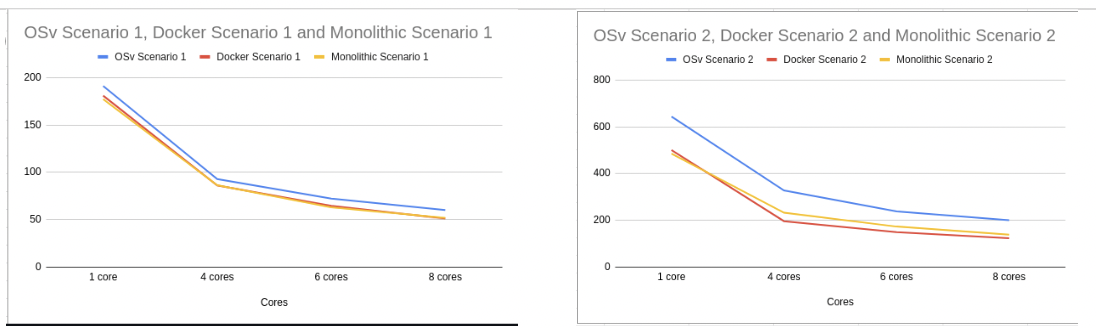
\includegraphics[width=2.54\textwidth]{WallClockRunTimes.png}
%      \end{tikzfigure}
%    \end{minipage}
%    \hspace{0.8cm}

%    \vspace{0.8cm}
%    \begin{minipage}[t]{0.4\linewidth}
%     % \vspace{-0.9cm}
%     \textbf{\textit{Parallel Speedups}}
%     \begin{tikzfigure}{}
%       \includegraphics[width=2.54\textwidth]{ParallelSpeedups.png}
%     \end{tikzfigure}
%   \end{minipage}

%   \vspace{0.8cm}
%   \begin{minipage}[t]{0.4\linewidth}
%     % \vspace{-0.9cm}
%     \textbf{\textit{Parallel Efficiency}}
%     \begin{tikzfigure}{}
%       \includegraphics[width=2.54\textwidth]{ParallelEffciency.png}
%     \end{tikzfigure}
%   \end{minipage}

%    % \hspace{0.2cm}

%    \begin{minipage}[t]{0.8\linewidth}

%    \end{minipage}%

%    \begin{tikzfigure}
%      % \includegraphics[width=0.4\textwidth]{images/parallel-layers-poster.png}
%    \end{tikzfigure}

%    \vspace{-2.5cm}
%  }

    % \NameBlock{model-checking}

  % \block{Conclusion}{
  %   \vspace{0.3cm}
  %   The empirical evidence gained from
  %   these measurements, running two different scenarios, will be used
  %   to answer the three research questions stated in the introduction
  %   of the paper. The empirical data from running the experiments on
  %   unikernels will provide a better understanding on how unikernels
  %   perform on a distributed memory environments.

  %   \vspace{1cm}

  %   \mbox{}\vspace{-\baselineskip}

  %   \printbibliography[heading=none]

  % }


\end{columns}

\begin{columns}


\column{1}

  \block{Architecture}{
    \vspace{0.7cm}
    \begin{minipage}[t]{0.4\linewidth}
      \vspace{-0.9cm}
      % \begin{tikzfigure}{}
      %   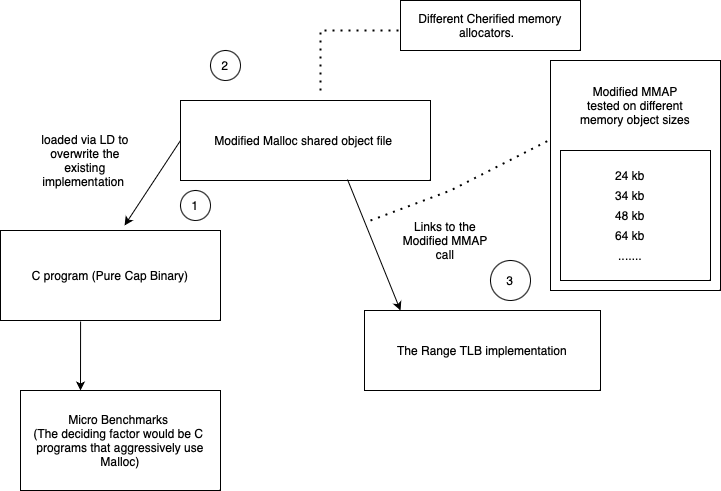
\includegraphics[width=2.53\textwidth]{Expirement-new.png}
      % \end{tikzfigure}
    \end{minipage}
    
    \vspace{0.5cm}
    % The above figure provides an higher overview of the expirement setup.
    % The expirement is divided into: 
    % \begin{itemize}
        % \item \textit{A set of Microbenchmarks which are designed
        % to create pressure on the L1 TLB to create more L1 misses.}
        % \item \textit{Modified Malloc to call the new syscall mmap\_range for large memory objects.}
        % \item \textit{Testing different memory object sizes to use the range TLB.}
    % \end{itemize}
}

  \end{columns}

\end{document}
